\begin{frame}
\frametitle{Recall the 1D toy model?}

\only<1|handout:4>{
\begin{itemize}
  \item exponential kernel: $K(s,t) = e^{-|s-t|/\lambda}$
  \item prescribed relative error $\varepsilon=10^{-4}$;
  \item \textbf{HODLR} admissibility;
  \item 1D exponential kernel: provably rank-one when \textbf{HODLR}.
  \item 'exact model' is the second Hermite function $\psi_2(x) = (2x^2-1)e^{-\frac{1}{2}x}$;
  \item input data as a gaussian distribution;
  \item here: one iteration of optimization loop, correlation length $\lambda=0.01$.
\end{itemize}
}

\only<2|handout:4>{
\begin{figure}[H]
\begin{center}
  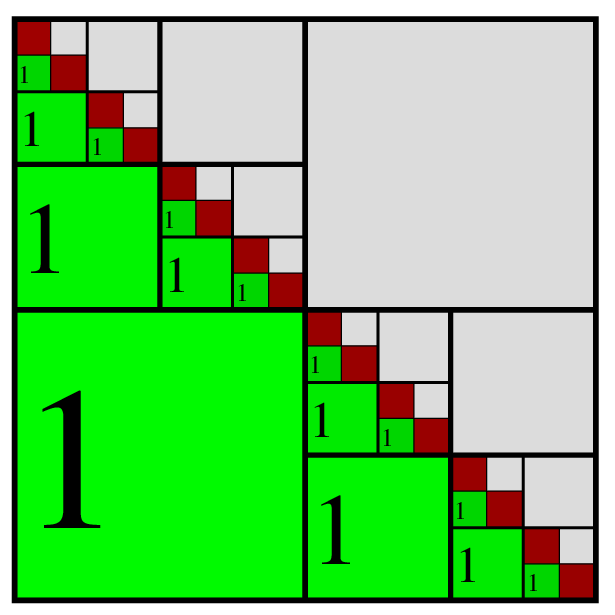
\includegraphics[scale=0.23]{./img/hmatrix-exp1d-assembled}
  \caption{Lower part of the covariance matrix: rank map.}
\end{center}
\end{figure}
\begin{itemize}
\item matrix size $1000 \times 1000$;
\item compression ratio: $\approx 12\%$ \textcolor{red}{(small case!)}
\end{itemize}
}

\only<3|handout:4>{
\begin{figure}[H]
\begin{center}
  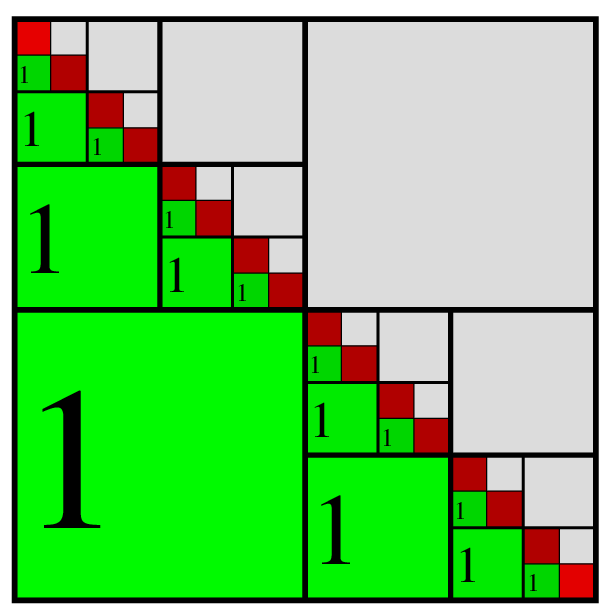
\includegraphics[scale=0.23]{./img/hmatrix-exp1d-factorized}
  \caption{Cholesky factor: rank map.}
\end{center}
\end{figure}
\begin{itemize}
\item matrix size $1000 \times 1000$;
\item compression ratio: $\approx 12\%$ \textcolor{red}{(small case!)}
\end{itemize}
}

\only<4|handout:4>{
\begin{figure}[H]
\begin{center}
  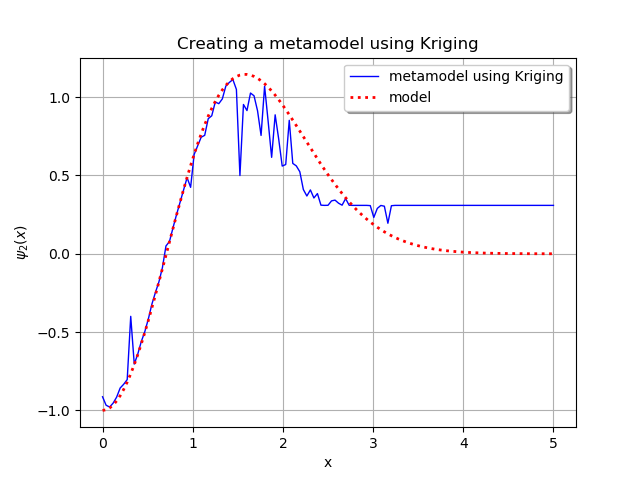
\includegraphics[scale=0.35]{./img/krigingResponse1d}
  \caption{Surface response using kriging}
\end{center}
\end{figure}

\begin{itemize}
\item compression ratio: $\approx 12\%$ \textcolor{red}{(small case!)};
\item same response with LAPACK and HMAT solver;
\item maximum absolute error between two approximates: $1.55 \times 10^{-15}$.
\end{itemize}
}
\end{frame}

